% =====================================================================
%  Effort Routing for CPU-Bound On-Device LLM Agents
%  arXiv draft (paper 2 of 2)  --  Bapista Khan / Collab-Foundry / NeuronAI
%
%  BUILD:  pdflatex main ; bibtex main ; pdflatex main ; pdflatex main
%  Needs pgfplots (TeX Live). No Python needed.
%
%  Companion to paper 1 ("Prefill Is the Bottleneck", \cite{khan2026prefill}):
%  paper 1 = the problem (prefill dominates CPU latency); this = the system.
%
%  Numbers below are from NeuronAI development logs (DESIGN_effort_router.md,
%  2026-06-21/22), warm, single runs, on the same Ryzen 7 8845HS box.
%  Red [FILL]/\note = controlled re-runs + reps still owed (Sec. Limitations).
%  These are real measurements, not fabricated; they need a clean re-run
%  under a fixed protocol before submission.
% =====================================================================
\documentclass[10pt,twocolumn]{article}

\usepackage[utf8]{inputenc}
\usepackage[T1]{fontenc}
\usepackage[margin=0.85in]{geometry}
\usepackage{graphicx}
\usepackage{booktabs}
\usepackage{amsmath,amssymb}
\usepackage{xcolor}
\usepackage[numbers,sort&compress]{natbib}
\usepackage[hidelinks]{hyperref}
\usepackage{caption}
\usepackage{pgfplots}
\pgfplotsset{compat=1.18}
\usepackage{algorithm}
\usepackage{algpseudocode}

\newcommand{\FILL}[1]{\textcolor{red}{[FILL: #1]}}
\newcommand{\note}[1]{\textcolor{blue}{\small$\blacktriangleright$#1}}

\title{\textbf{Spend Cognition, Not Parameters: Effort Routing for
CPU-Bound On-Device LLM Agents}}

\author{
  Bapista Khan\\
  Collab-Foundry / NeuronAI\\
  \texttt{bapistakhan@gmail.com}
}
\date{July 2026}

\begin{document}
\maketitle

% =====================================================================
\begin{abstract}
\noindent
On CPU-only on-device deployment, prefill---not decode---dominates LLM
latency, and that cost scales with prompt length~\cite{khan2026prefill}.
Yet a typical agent runs its full stack (context injection, a
review/verify second model pass, grounding, post-refinement) on every
query, paying that prefill cost even for trivial inputs. We present an
\emph{effort router} for on-device LLM agents that routes the \emph{depth
of cognition} (and specialist troop), not the model size, keeping a
$\geq$7B model on every path. Three lanes---Reflex, Standard, Deep---gate
expensive stages by request difficulty using a pure-heuristic classifier
(no extra model call). On a 14~GiB Ryzen~7 8845HS (CPU-only), the router
cuts trivial ``reflex'' queries from 14--25~s to 1.4--6.7~s, plain
Standard queries from 90.9~s to 22.1~s, and knowledge (RAG) Standard
queries from 143.5~s to 54.7~s. Our most useful finding is
counterintuitive: the dominant Standard-lane cost was not prompt length
but an \emph{extra review model pass}; gating it to the Deep lane alone cut
plain-Standard latency $\sim$4$\times$, with no measurable quality loss in a
controlled order-swapped LLM-judge test (revised answers won 1/8, tied
7/8). We also identify a model-eviction
pathology under single-slot loading that silently added $\sim$45~s per RAG
query.
\end{abstract}

% =====================================================================
\section{Introduction}
\label{sec:intro}

Sovereign, offline-first agents increasingly run LLMs on commodity CPUs.
In this regime, prefill (reading the prompt) dominates end-to-end
latency---exceeding 90\% at realistic prompt lengths on
CPU~\cite{khan2026prefill}. A companion consequence, which this paper
addresses, is that a conventional agent pipeline pays that cost
indiscriminately: every query, however trivial, runs context injection, a
review/verify pass, grounding, and post-refinement on a 7--9B model.

We argue the right response on CPU is to \emph{route effort}, not model
size. A sub-7B ``router model'' would lower quality and still pay a model
call; instead we route the \emph{depth of cognition}---how many pipeline
stages run---and the specialist troop, keeping a $\geq$7B floor everywhere.
Contributions:
\begin{enumerate}
  \item An effort-routing architecture with three difficulty lanes and a
        pure-heuristic (model-free) classifier (Section~\ref{sec:design}).
  \item Five prefill-aware latency levers---hot-model affinity, per-lane
        prompt/context budgeting, review-pass gating, per-lane generation
        caps, and shared-prefix condensation---each tied to the prefill
        finding (Section~\ref{sec:design}).
  \item An evaluation on CPU-only hardware showing 2--6$\times$ latency
        reductions per lane, and two non-obvious findings: (i) an extra
        \emph{review model pass}, not prompt length, was the dominant
        Standard cost; (ii) single-slot model loading caused a
        chat$\leftrightarrow$embedder eviction that added $\sim$45~s per
        RAG query (Section~\ref{sec:eval}).
\end{enumerate}

\noindent\textbf{Scope.} Single-machine, CPU-only, one runtime, a fleet of
7--9B quantized models. Numbers are from the deployed system's development
logs; a controlled re-run protocol is future work
(Section~\ref{sec:limitations}).

% =====================================================================
\section{Background}
\label{sec:background}

\paragraph{Prefill-bound CPU inference.}
On CPU there is little parallelism to hide prefill's per-token compute, so
latency tracks \emph{context length}, not output length~\cite{khan2026prefill}.
Every system-prompt token, governance rule, and retrieved passage is paid
for at the prefill rate ($\sim$46~tok/s on our box) before the first output
token.

\paragraph{Single-slot loading.}
Under a memory-constrained runtime (\texttt{OLLAMA\_MAX\_LOADED\_MODELS}),
switching models forces a multi-second cold reload (a 7--9B load is
$\sim$5--6~GB, $\sim$65~s). Per-query model switching is therefore a
latency hazard the router must avoid.

\paragraph{The stock pipeline.}
The baseline agent runs, per query: awareness/context injection $\to$ a
review/verify \emph{second} model pass $\to$ grounding $\to$
post-refinement, on a 7--9B model. Every stage adds prompt (prefill) or an
extra generation (decode) cost.

% =====================================================================
\section{Design: The Effort Router}
\label{sec:design}

\paragraph{Principles.}
(P1) \textbf{7B floor} on every lane---route effort, never below the
quality floor. (P2) \textbf{Hot-model affinity}---prefer the resident
model; pay a reload only when the expected quality gain clears a budget.
(P3) \textbf{Spend cognition where it pays}---trivial$\to$minimal,
substantive$\to$full, hard$\to$escalate. (P4) \textbf{Routing is
$\sim$free}---pure heuristics; a model classifier would itself need the
7B.

\paragraph{Three lanes.}
Table~\ref{tab:lanes} defines the lanes. A cheap heuristic
(\texttt{\_classify\_lane}) inspects length, punctuation, question-worthiness,
and keyword/domain cues; \texttt{/think} forces Deep; ambiguous cases bias
to Standard.

\begin{table}[t]
  \centering
  \caption{The three effort lanes. All run a $\geq$7B model.}
  \label{tab:lanes}
  \small
  \begin{tabular}{lp{3.1cm}l}
    \toprule
    Lane & Trigger (heuristic) & Stages \\
    \midrule
    Reflex   & greeting/ack, time, identity, very short, non-question & lite awareness; \emph{skip} review/grounding/refine \\
    Standard & normal substantive question & full stack; review only if warranted \\
    Deep     & long / \texttt{/think} / multi-part / legal$\cdot$code$\cdot$math keywords & full stack + forced revise + verify pass \\
    \bottomrule
  \end{tabular}
\end{table}

\paragraph{Latency levers (all prefill-aware).}
\begin{itemize}
  \item \textbf{Hot-model affinity.} If the best-fit troop $\neq$ resident
        model and the domain match is weak and the lane is not Deep,
        override to the resident generalist---avoiding a $\sim$65~s reload.
  \item \textbf{Per-lane prompt/context budget.} Cap awareness/RAG context
        by lane (Standard $\sim$3{,}000 chars; Deep $\sim$16{,}000), since
        latency tracks prompt length.
  \item \textbf{Review-pass gating.} Restrict the expensive review/verify
        \emph{second model pass} to the Deep lane---the single highest-
        leverage change (Section~\ref{sec:eval}).
  \item \textbf{Per-lane generation cap.} Bound output tokens by lane
        (Reflex 64 / Deep 768) to remove uncapped-generation variance.
  \item \textbf{Shared-prefix condensation.} Condense the persona/governance
        boilerplate at the source (e.g.\ the 10 numbered governance rules
        instead of the full rule table), shrinking the shared prefix on
        \emph{every} prompt ($\sim$1{,}000 chars saved per prompt; identity
        prompt 4{,}280$\to$3{,}209 chars).
\end{itemize}

\paragraph{Implementation.}
\texttt{\_route\_effort} returns \texttt{\{lane, troop, model, flags\}} and
is called before the CEO prepare step; Reflex short-circuits there. Stage
gating is consumed by the streaming path to skip review/grounding/refine on
fast lanes. Algorithm~\ref{alg:route} gives the pure-heuristic classifier and
the hot-affinity arbitration; both are model-free and unit-tested.

\begin{algorithm}[t]
\caption{Effort routing: model-free lane classification (\textsc{ClassifyLane})
and hot-affinity model arbitration (\textsc{RouteEffort}). $G$ is the resident
7B generalist; $hot$ is the currently loaded model ($\varnothing$ if none).}
\label{alg:route}
\small
\begin{algorithmic}[1]
\Procedure{ClassifyLane}{$q$}\Comment{no model call}
  \If{$q$ begins with \texttt{/think} or \texttt{/deep}}
     \State \Return \textsc{deep}
  \EndIf
  \State $w \gets$ number of words in $q$
  \If{$w \le 10$ \textbf{and} $q$ matches a greeting/ack, identity,
      or time pattern}
     \State \Return \textsc{reflex}
  \EndIf
  \If{$w > 80$ \textbf{or} $q$ has ${\ge}\,2$ question marks \textbf{or}
      $q$ matches a hard-signal pattern}
     \Statex \hfill{\footnotesize(legal, debug, prove, analyse, compare, design, \dots)}
     \State \Return \textsc{deep}
  \EndIf
  \State \Return \textsc{standard}\Comment{ambiguous biases here}
\EndProcedure
\Statex
\Procedure{RouteEffort}{$q$, $hot$}
  \State $\ell \gets \Call{ClassifyLane}{q}$
  \If{$\ell = \textsc{reflex}$ \textbf{and} $q$ is not a web task}
     \State $m \gets hot$ \textbf{if} $hot$ is a non-embedder \textbf{else} $G$
     \State \Return generalist troop, model $m$, \emph{skip} review/grounding
  \EndIf
  \State $prep \gets \Call{CommandPrepare}{q}$\Comment{best-fit specialist troop+model}
  \If{$\ell \ne \textsc{deep}$ \textbf{and} $hot \ne \varnothing$ \textbf{and}
      $hot$ is a non-embedder \textbf{and} $prep.\textit{model} \ne hot$}
     \State $prep.\textit{model} \gets hot$\Comment{avoid a ${\sim}65$\,s reload}
  \EndIf
  \State $prep.\textit{review} \gets (\ell = \textsc{deep})$\Comment{review pass: Deep only}
  \State \Return $prep$
\EndProcedure
\end{algorithmic}
\end{algorithm}

% =====================================================================
\section{Evaluation}
\label{sec:eval}

\paragraph{Setup.}
Same platform as~\cite{khan2026prefill}: AMD Ryzen~7 8845HS (8C/16T),
14~GiB shared memory, CPU-only, Ollama (llama.cpp), generalist
Qwen2.5-7B~(Q4) with per-domain 7--9B troops. Latencies are warm
(model resident), from the deployed system's development logs.
\note{The per-lane table is from development logs; the review-pass lever is
additionally validated in a controlled matched experiment
(Table~\ref{tab:reviewpass}). A full per-lane re-run with $\geq$5 reps +
error bars is still owed (Sec.~\ref{sec:limitations}).}

\paragraph{Per-lane results.}
Table~\ref{tab:results} and Figure~\ref{fig:bars} show end-to-end latency
before and after routing, per lane.

\begin{table}[t]
  \centering
  \caption{End-to-end latency by lane, before vs.\ after effort routing
  (warm, CPU-only). Development-log measurements.}
  \label{tab:results}
  \small
  \begin{tabular}{llrr}
    \toprule
    Lane & Example query & Before & After \\
    \midrule
    Reflex            & ``thanks!''                & 14--25\,s & 4.5\,s \\
    Standard (plain)  & ``benefit of unit tests''  & 90.9\,s   & 22.1\,s \\
    Standard (RAG)    & ``what is photosynthesis'' & 143.5\,s  & 54.7\,s \\
    Standard (RAG)    & name-benefit query         & 66\,s     & 44.8\,s \\
    Deep              & ``\texttt{/think} REST vs GraphQL'' & 190\,s & 104\,s \\
    \bottomrule
  \end{tabular}
\end{table}

\begin{figure}[t]
  \centering
  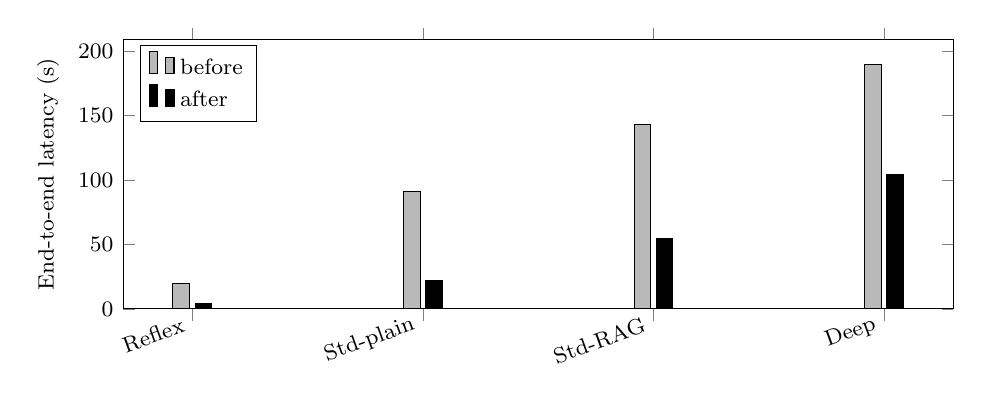
\begin{tikzpicture}
    \begin{axis}[
      width=\columnwidth, height=5.0cm,
      ybar, bar width=6pt,
      symbolic x coords={Reflex, Std-plain, Std-RAG, Deep},
      xtick=data, x tick label style={font=\footnotesize, rotate=20, anchor=east},
      ylabel={End-to-end latency (s)}, ymin=0,
      label style={font=\footnotesize}, tick label style={font=\footnotesize},
      legend style={font=\footnotesize, at={(0.02,0.98)}, anchor=north west},
      legend cell align=left,
    ]
      \addplot[fill=gray!55] coordinates
        {(Reflex,20) (Std-plain,90.9) (Std-RAG,143.5) (Deep,190)};
      \addplot[fill=black] coordinates
        {(Reflex,4.5) (Std-plain,22.1) (Std-RAG,54.7) (Deep,104)};
      \legend{before, after}
    \end{axis}
  \end{tikzpicture}
  \caption{Latency before vs.\ after effort routing, per lane (CPU-only).
  2--6$\times$ reductions.}
  \label{fig:bars}
\end{figure}

\paragraph{Finding 1: the review pass, not prompt length, dominated.}
Budgeting the prompt alone barely moved plain Standard. The dominant cost
was the review/verify \emph{second model pass}---a whole extra
generation---left on for Standard. Restricting it to Deep cut plain
Standard $\sim$4$\times$ (90.9$\to$22.1~s). Prompt budgeting helped the
RAG/knowledge case, where retrieved context inflates prefill.

\paragraph{Controlled review-pass isolation (latency + quality).}
To isolate the review pass from heterogeneous dev-log conditions, we ran a
matched experiment: 8 factual queries, each answered single-pass and then
two-pass (answer $+$ review/revise), warm Qwen2.5-7B~(Q4), one run each at
temperature~0 (Table~\ref{tab:reviewpass}). The review pass raised latency
\textbf{2.41$\times$} ($11.96\to28.79$~s). For quality we asked an
LLM-judge---run in \emph{both} orders per query to cancel position
bias---whether the revised answer beat the single-pass one: it did in only
\textbf{1 of 8} cases, tied in 7, and was worse in none. The review pass
thus more than doubles latency for a quality gain undetectable on standard
factual queries, directly justifying its gating to the Deep lane. (The
judge is an LLM on relatively easy prompts; harder or generative queries
may benefit more, which is why Deep retains the pass.)

\begin{table}[t]
  \centering
  \caption{Controlled review-pass isolation: single- vs.\ two-pass latency
  and order-swapped LLM-judge quality, over 8 matched queries (warm,
  Qwen2.5-7B Q4, CPU-only). Std is across queries.}
  \label{tab:reviewpass}
  \small
  \begin{tabular}{lr}
    \toprule
    Metric & Value \\
    \midrule
    Single-pass latency (s)       & 11.96$\pm$5.49 \\
    Two-pass latency (s)          & 28.79$\pm$12.84 \\
    Review-pass overhead          & 2.41$\times$ \\
    \midrule
    Revised answer judged better  & 1 / 8 \\
    Tie                           & 7 / 8 \\
    Single-pass judged better     & 0 / 8 \\
    \bottomrule
  \end{tabular}
\end{table}

\paragraph{Finding 2: single-slot eviction added $\sim$45~s.}
Under single-slot loading, every RAG query evicted the chat model to load
the embedder, then reloaded chat from disk---an unbudgeted $\sim$45~s
penalty. Allowing two resident models
(\texttt{OLLAMA\_MAX\_LOADED\_MODELS}=2, $\sim$5~GB total) let them
coexist, cutting knowledge-Standard 85.9$\to$54.7~s. This is safe only
because hot-affinity and the memory guard prevent a two-large-model swap.

\paragraph{Cumulative effect.}
Knowledge-Standard fell across the work: 143~s $\to$ 75~s (single-pass
review gating) $\to$ 54~s (two-slot loading). The residual is genuine RAG
retrieval + prefill + longer generation.

% =====================================================================
\section{Discussion}
\label{sec:discussion}

\paragraph{Why it works.}
Every lever targets the prefill-bound cost model~\cite{khan2026prefill}:
hot-affinity avoids re-prefilling after a reload; prompt/prefix budgets
shrink the prefilled context; review-pass gating removes an entire extra
prefill+decode; generation caps bound decode variance. Routing effort
rather than model size keeps quality at the 7B floor while spending
compute only where difficulty warrants.

\paragraph{Tradeoffs (stated plainly).}
Standard queries skip the post-hoc verification pass; full verification is
the opt-in Deep lane. Shared-prefix condensation's warm same-troop win is
modest ($\sim$5~s) because the runtime caches the shared prompt prefix---the
real payoff is on troop switches, cold starts, and memory footprint.
Misclassification risk (a Deep query labelled Reflex) is mitigated by
biasing ambiguous cases to Standard and letting \texttt{/think} force Deep.

% =====================================================================
\section{Limitations}
\label{sec:limitations}
The per-lane latencies (Table~\ref{tab:results}) are from development logs:
warm, single runs, heterogeneous query strings, one machine, one runtime.
The review-pass lever is validated separately in a controlled matched
experiment with an order-swapped LLM-judge (Section~\ref{sec:eval},
Table~\ref{tab:reviewpass}), which found no quality regression from gating
it. Before submission we will extend this to a full per-lane re-run
($\geq$5 reps, error bars, matched queries per lane, warm and cold) and a
broader quality set (harder and generative prompts, ideally with human
labels). We do not evaluate multi-user serving.

% =====================================================================
\section{Related Work}
\label{sec:related}
LLM routing and cascades reduce cost by sending easy queries to cheaper
models~\cite{chen2023frugalgpt, ong2024routellm}; we differ by keeping a
fixed $\geq$7B model and routing \emph{pipeline effort} on a single CPU
device, motivated by the prefill cost model. Serving systems optimize the
prefill/decode split on GPUs~\cite{kwon2023pagedattention,
agrawal2024sarathi}; we operate single-user on CPU. On-device inference
surveys~\cite{xu2024ondevicereview} catalogue compression and runtime
levers; our contribution is a request-adaptive \emph{pipeline} policy.
Our lane gating is a coarse, pipeline-level analogue of \emph{adaptive
computation}: where confident adaptive language
modeling~\cite{schuster2022calm} exits the decoder early per token, we skip
whole pipeline stages per request, keeping a fixed model. \emph{Speculative
decoding}~\cite{leviathan2023speculative} instead accelerates the decode
phase itself; it is complementary and orthogonal to our prefill-motivated,
stage-level routing. Finally, we use an LLM as an automatic quality
judge~\cite{zheng2023judging} to check that gating the review pass causes no
regression (Section~\ref{sec:eval}); we mitigate its known position bias by
running each comparison in both orders.

% =====================================================================
\section{Conclusion}
\label{sec:conclusion}
On CPU-only on-device deployment, where prefill dominates, routing effort
rather than model size yields 2--6$\times$ latency reductions without
lowering the model floor. The highest-leverage change was removing an
extra review model pass from the common path---a reminder that on CPU, the
cheapest token is the one never prefilled or generated.

% =====================================================================
\section*{Reproducibility}
\label{sec:repro}
The controlled review-pass harness (\texttt{review\_pass\_experiment.py})
and its raw results (\texttt{review\_pass\_results.json}) are released at
\url{https://github.com/bapista/cpu-llm-latency} (directory
\texttt{paper2/data/}), alongside the companion prefill study
(\texttt{paper1/}), and mirrored in the arXiv ancillary files.

% =====================================================================
\bibliographystyle{plainnat}
\bibliography{references}

\end{document}
